\documentclass{beamer}
\usepackage{beamerthemesplit}
\usepackage{wrapfig}
\usetheme{SPbGU}
\usepackage{pdfpages}
\usepackage{amsmath}
\usepackage{mathtools}
\usepackage{cmap} 
\usepackage[T2A]{fontenc} 
\usepackage[utf8]{inputenc}
\usepackage[english,russian]{babel}
\usepackage{indentfirst}
\usepackage{amsmath}
\usepackage{tikz}
\usepackage{multirow}
\usepackage[noend]{algpseudocode}
\usepackage{algorithm}
\usepackage{algorithmicx}
\usetikzlibrary{shapes,arrows}
\usepackage{fancyvrb}
\newtheorem{rutheorem}{Теорема}
\newtheorem{ruproof}{Доказательство}
\newtheorem{rudefinition}{Определение}
\newtheorem{rulemma}{Лемма}
\beamertemplatenavigationsymbolsempty

\title[]{Теория автоматов и формальных языков}
\subtitle[]{Регулярные языки}
\institute[]{
Санкт-Петербургский государственный электротехнический университет <<ЛЭТИ>>\\
}

\author[]{Екатерина Вербицкая}

\date{ сентября 2016г.}

\definecolor{orange}{RGB}{179,36,31}

\begin{document}
{
  \begin{frame}
    \titlepage
  \end{frame}
}

\begin{frame}[fragile]
  \transwipe[direction=90]
  \frametitle{Регулярная грамматика}
  \textbf{Праволинейная грамматика} --- грамматика, все правила которой имеют следующий вид:
  \begin{itemize}
    \item $A \rightarrow \omega B$ или $A \rightarrow \omega$, где $A, B \in V_N, \omega \in V^*$
  \end{itemize}


  \textbf{Леволинейная грамматика} --- грамматика, все правила которой имеют следующий вид:
  \begin{itemize}
    \item $A \rightarrow B \omega$ или $A \rightarrow \omega$, где $A, B \in V_N, \omega \in V^*$
  \end{itemize}

\pause 

  \begin{rutheorem}[]
    Пусть L --- формальный язык. 

    $\exists G_r$ --- праволинейная грамматика, т.ч. $L = L(G_r) \Leftrightarrow \exists G_l$ --- леволинейная грамматика, т.ч. $L = L(G_l) $
  \end{rutheorem}
\pause
  \textbf{Регулярная грамматика} --- праволинейная или леволинейная грамматика
\end{frame}

\begin{frame}[fragile]
  \transwipe[direction=90]
  \frametitle{Конечный автомат}
  \textbf{Конечный автомат} --- $\langle Q, \Sigma, \delta, q_0, F \rangle$
  \begin{itemize}
    \item $Q \neq \emptyset$ --- конечное множество состояний
    \item $\Sigma$ --- Конечный входной алфавит
    \item $\delta$ --- отображение типа $Q \times \Sigma \rightarrow Q$
    \item $q_0 \in Q$ --- начальное состояние
    \item $F \subseteq Q$ --- множество конечных состояний
  \end{itemize}
\end{frame}


\begin{frame}[fragile]
  \transwipe[direction=90]
  \frametitle{Пример конечного автомата}

 $Q = \{ 0, 1, 2, 3\}, \Sigma = \{ 0, 1, -\}, q_0 = 0, F = \{1, 2\}$
 
 $\delta (0, 0) = 1; \delta (0, 1) = 2; \delta (0, -) = 3; \delta (3, 1) = 2; \delta (2, 0) = 2; \delta (2, 1) = 2 $ 

  \begin{center}
     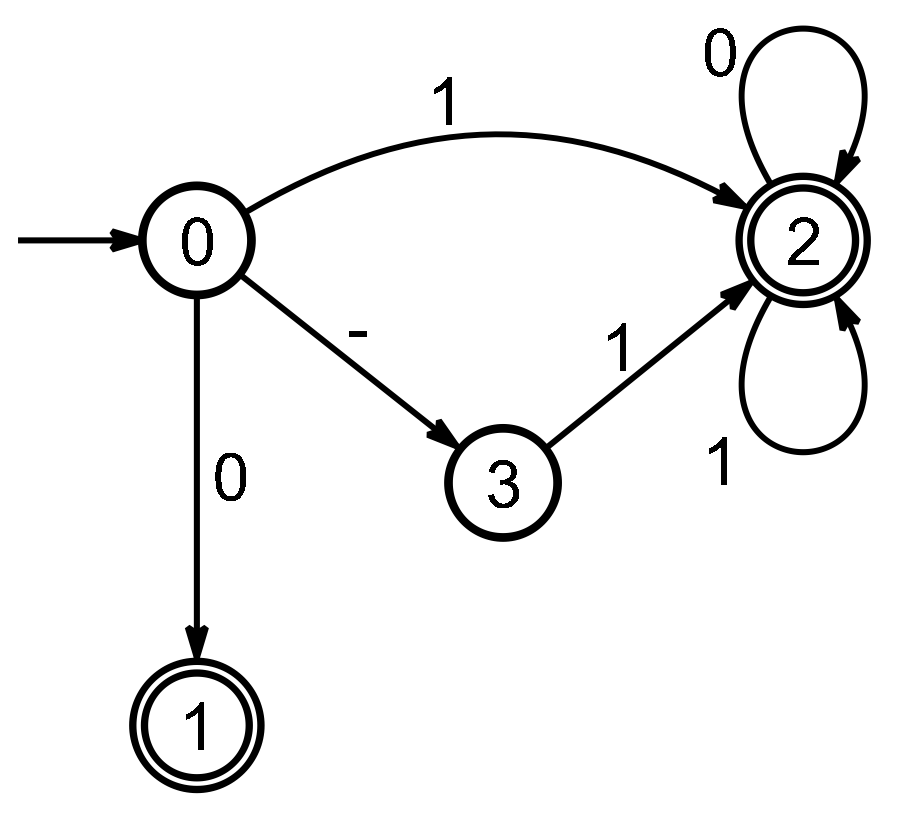
\includegraphics[width=0.55\textwidth]{pics/automaton.png}  
   \end{center}
\end{frame}


\begin{frame}[fragile]
  \transwipe[direction=90]
  \frametitle{Распознавание слова конечным автоматом}
  \begin{itemize}
    \item  Обобщаем функцию перехода: 
    \begin{itemize}
      \item $\delta' (q, \varepsilon) = q$
      \item $\delta' (q, xa) = \delta(\delta'(q, x), a)$, где $x \in \Sigma^*, a \in \Sigma$
    \end{itemize}
    \item Цепочка $\omega$ \textbf{распознается} конечным автоматом $\langle Q, \Sigma, \delta, q_0, F \rangle$, если $\exists p \in P. \delta'(q, \omega) = p$
    \item \textbf{Язык, распознаваемый конечным автоматом}: $\{ \omega \in \Sigma^* \, | \, \exists p \in F.\delta'(q_0, \omega) = p \}$
  \end{itemize}
\end{frame}

\begin{frame}[fragile]
  \transwipe[direction=90]
  \frametitle{Минимальный конечный автомат}
  \begin{itemize}
    \item Конечные автоматы $A_1$ и $A_2$ \textbf{эквивалентны}, если распознают один и тот же язык
    \item \textbf{Минимальный конечный автомат} --- автомат, имеющий наименьшее число состояний, распознающий тот же язык, что и данный
  \end{itemize}
\end{frame}

\begin{frame}[fragile]
  \transwipe[direction=90]
  \frametitle{Классы эквивалентности}
    \textbf{Отношение эквивалентности} --- рефлексивное, симметричное, транзитивное отношение
    \begin{itemize}
      \item $xRx; xRy \Leftrightarrow yRx; xRy, yRz \Rightarrow xRz$
    \end{itemize}
    
    \begin{rutheorem}
       $\forall R$ --- отношение эквивалентности на множестве $S$
      
      Можно разбить $S$ на $k$ непересекающихся подмножеств $I_1 \dots I_k$, т.ч. $aRb \Leftrightarrow a, b \in I_j$
    \end{rutheorem}
    
    Множества $I_1 \dots I_k$ называются \textbf{классами эквивалентности}
\end{frame}

\begin{frame}[fragile]
  \transwipe[direction=90]
  \frametitle{Эквивалентные состояния}
  \begin{itemize}
    \item $\omega \in \Sigma^*$ различает состояния $q_i$ и $q_j$, если $\delta' (q_i, \omega) = t_1, \delta' (q_j, \omega) = t_2 \Rightarrow (t_1 \notin F \Leftrightarrow t_2 \in F)$
    \item $q_i$ и $q_j$ \textbf{эквивалентны} $(q_i \sim q_j)$, если $\forall \omega \in \Sigma^*. \delta' (q_i, \omega) = t_1, \delta' (q_j, \omega) = t_2 \Rightarrow (t_1 \in F \Leftrightarrow t_2 \in F)$
    \begin{itemize}
      \item Является отношением эквивалентности
    \end{itemize}
  \end{itemize}
   \begin{rulemma}
      $\mathcal{A} = \langle Q, \Sigma, \delta, q_0, F \rangle, p_1, p_2, q_1, q_2 \in Q, q_i = \delta(p_i, c)$
      
      $\omega \in \Sigma^*$ различает $q_1$ и $q_2$. Тогда $c \omega$ различает $p_1$ и $p_2$
   \end{rulemma}
   
   \begin{ruproof}
     $\delta' $
   \end{ruproof}
\end{frame}

\begin{frame}[fragile]
  \transwipe[direction=90]
  \frametitle{}
  \begin{itemize}
    \item 
  \end{itemize}
\end{frame}

\begin{frame}[fragile]
  \transwipe[direction=90]
  \frametitle{}
  \begin{itemize}
    \item 
  \end{itemize}
\end{frame}

\begin{frame}[fragile]
  \transwipe[direction=90]
  \frametitle{}
  \begin{itemize}
    \item 
  \end{itemize}
\end{frame}

\begin{frame}[fragile]
  \transwipe[direction=90]
  \frametitle{}
  \begin{itemize}
    \item 
  \end{itemize}
\end{frame}

\begin{frame}[fragile]
  \transwipe[direction=90]
  \frametitle{}
  \begin{itemize}
    \item 
  \end{itemize}
\end{frame}

\begin{frame}[fragile]
  \transwipe[direction=90]
  \frametitle{}
  \begin{itemize}
    \item 
  \end{itemize}
\end{frame}

\begin{frame}[fragile]
  \transwipe[direction=90]
  \frametitle{}
  \begin{itemize}
    \item 
  \end{itemize}
\end{frame}

\begin{frame}[fragile]
  \transwipe[direction=90]
  \frametitle{}
  \begin{itemize}
    \item 
  \end{itemize}
\end{frame}

\begin{frame}[fragile]
  \transwipe[direction=90]
  \frametitle{}
  \begin{itemize}
    \item 
  \end{itemize}
\end{frame}

\begin{frame}[fragile]
  \transwipe[direction=90]
  \frametitle{}
  \begin{itemize}
    \item 
  \end{itemize}
\end{frame}

\begin{frame}[fragile]
  \transwipe[direction=90]
  \frametitle{}
  \begin{itemize}
    \item 
  \end{itemize}
\end{frame}

\end{document}
